\documentclass[tikz]{standalone}

\usepackage{pgfplots}
\pgfplotsset{compat=1.18}

\begin{document}
  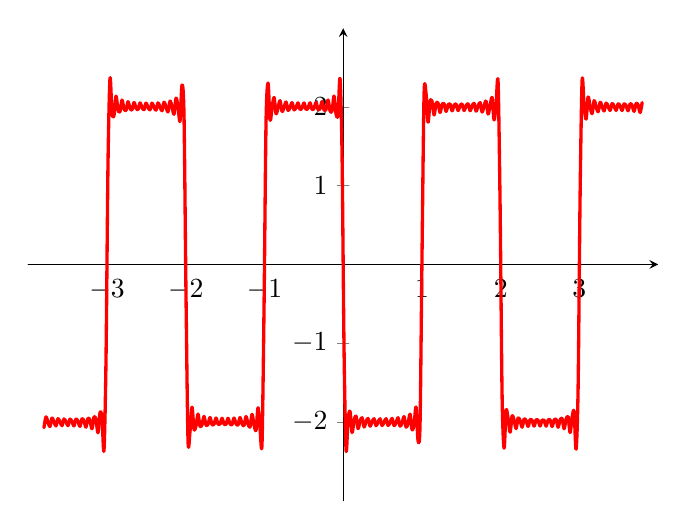
\begin{tikzpicture}[line cap=round,line join=round]
    \begin{axis}[
    x=1.0cm,y=1.0cm,
    axis lines=middle,
    xmin=-4,
    xmax=4,
    ymin=-3,
    ymax=3,
    xtick={-3.0,-2.0,...,3.0},
    ytick={-2.0,-1.0,...,2.0},]
      % Plot obtenido desde geogebra
      \draw[very thick,red,smooth,samples=300,domain=-3.8:3.8] plot(\x,{
        -2.55*(
        sin((\x)*180)+
        sin(((3)*(\x))*180)/(3)+
        sin(((5)*(\x))*180)/(5)+
        sin(((7)*(\x))*180)/(7)+
        sin(((9)*(\x))*180)/(9)+
        sin(((11)*(\x))*180)/(11)+
        sin(((13)*(\x))*180)/(13)+
        sin(((15)*(\x))*180)/(15)+
        sin(((17)*(\x))*180)/(17)+
        sin(((19)*(\x))*180)/(19)+
        sin(((21)*(\x))*180)/(21)+
        sin(((23)*(\x))*180)/(23)+
        sin(((25)*(\x))*180)/(25)
        )
      });
    \end{axis}
  \end{tikzpicture}
\end{document}
